
\section{Definitions}

A grid edge, facet or cube is {\em active} if it contains at least one vertex 
with scalar value greater than or equal to the isovalue
and at least one vertex with scalar value less than the isovalue.

A grid cube with grid indices $(x_0,x_1,x_2)$ is in column $x_0$, row $x_1$
and $z$-plane $x_2$ of the grid.
Let $\cb$ and $\cb'$ be grid cubes with grid indices $(x_0,x_1,x_2)$
and $(x'_0,x'_1,x'_2)$, respectively.
The {\em cube distance} between the cubes 
is $\max(|x_0-x'_0|, |x_1-x'_1|, |x_2-x'_2|)$.
The {\em distance vector} between the cubes is
$(|x_0-x'_0|, |x_1-x'_1|, |x_2-x'_2|)$.

For a grid cube $\cb$, region $\RIII_\cb$ is the $3 \times 3 \times 3$ region
of 27 grid cubes centered at $\cb$.
Region $\RV_\cb$ is the $5 \times 5 \times 5$ region
of 125 grid cubes centered at $\cb$.


\section{Computing Isosurface Vertex Locations}
\label{section:loc}

At the heart of any algorithm to compute a surface with sharp features 
is an algorithm to compute the locations of mesh vertices on those features.
In order to understand some of the problems in MergeSharp 
and the improvements in this paper,
it is necessary to understand this algorithm for computing vertex locations.
We review that algorithm here.

Mergesharp computes one isosurface vertex location $p_\cb$
for each active grid cube $\cb$.
The algorithm computes an isosurface vertex location for $\cb$
by using the gradients at vertices of $\cb$ and neighboring cubes.
If grid vertex $v_i$ has scalar $s_{v_i}$ and gradient $g_{v_i}$, 
then the plane tangent to the isosurface  with isovalue $\sigma$
is $\{p : (p-v_i) \cdot g_{v_i} + s_{v_i}= \sigma \}$.
A set of $k$ vertices and gradients gives a set of $k$ equations 
in three variables $M p = b$
where $M$ is a $k \times 3$ matrix 
and $b$ is a column vector with $k$ rows 
and the unknown $p$ is a column vector with three rows.
Of course, if $M$ has more than three rows,
the system $Mp = b$ is over-determined and has no exact solution.
The least squares approximation to $M p = b$ 
is the solution to $M^T M p = M^T b$.

Let $A$ be the $3 \times 3$ matrix $M^T M$ and 
let $b'$ equal the column vector $M^T b$.
MergeSharp uses singular valued decomposition (SVD)
as described in~\cite{jlsw-dchd-02,kbsh-fssev-01,l-oslpm-00}
to compute an isosurface vertex location from the equation $A p = b'$.

Let $\sigma_1$, $\sigma_2$ and $\sigma_3$ be the singular values of $A$
sorted in decreasing order.
A singular value $\sigma_i$ is {\em large},
if $\sigma_i/\sigma_1 \ge \epsilon$ for some predefined parameter $\epsilon$.
There are three possible cases based on the number of large singular values
of $A$.
In the first case $A$ has three large singular values.
In this case, the tangent planes around $\cb$ have normals in three or more
very distinct directions.
The isosurface has some sharp corner near cube $\cb$.
We call a cube $\cb$ a {\em corner cube} if the matrix $A$ associated
with $\cb$ has three large singular values.
The solution to $A p = b'$ approximates the corner point near cube $\cb$.

In the second case, matrix $A$ has only two large singular values.
In this case, 
the tangent plane normals are close to two different directions.
The isosurface has some sharp edge near cube $\cb$.
We call a cube $\cb$ an {\em edge cube} if the matrix $A$ associated
with $\cb$ has two large singular values.

To compute the sharp edge near $\cb$,
we use singular valued decomposition to remove the small singular value
from $A$.
The singular valued decomposition of $A$ is $A = U \Sigma V^T$
where
\begin{equation*}
\Sigma = \left (
\begin{array}{ccc}
\sigma_1 & 0 & 0 \\
0 & \sigma_2 & 0 \\
0 & 0 & \sigma_3
\end{array}
\right )
.
\end{equation*}
When $A$ has only two large singular values, $\sigma_1$ and $\sigma_2$,
MergeSharp replaces $\Sigma$ by a new diagonal matrix $\Sigma'$
with diagonal entries $\sigma_1$, $\sigma_2$, 0.
Let $A'$ equal $U \Sigma V^T$.
Matrix $A'$ has rank two.
The solution to $A' p = b'$ is a set of points on a line.
That line represents a line containing the sharp edge.

In the last case,
matrix $A$ has only one large singular value.
In this case, the tangent plane normals are close to a single direction.
The isosurface is smooth around cube $\cb$.
Replace $\Sigma$ by a new diagonal matrix $\Sigma'$
with diagonal entries $\sigma_1$, 0, 0.
Let $A'$ equal $U \Sigma V^T$.
Matrix $A'$ has rank one.
The solution to $A' p = b'$ is a set of points on a plane.
That plane represents a tangent plane to the isosurface in cube $\cb$.

In the case that $A$ has only one or two large singular values,
the solution to $A' p = b'$ is a line or plane.
Using linear interpolation,
MergeSharp approximates the intersection of each edge of $\cb$
and the isosurface and then computes the point $q_\cb$
at the centroid of those interpolated intersection points.
As suggested in~\cite{sw-dcss-02},
MergeSharp selects the point on the line or plane that is closest to $q_\cb$.

More precisely, MergeSharp defines the diagonal matrix $\Sigma^+$
with diagonal entries:
\begin{equation*}
\begin{array}{ll}
1/\sigma_1, 1/\sigma_2, 1/\sigma_3, 
  & \mbox{ if $A$ has three singular values,}\\
1/\sigma_1, 1/\sigma_2, 0, 
  & \mbox{ if $A$ has two singular values,}\\
1/\sigma_1, 0, 0, 
  & \mbox{ if $A$ has one singular value.}
\end{array}
\end{equation*}
The point
\begin{equation}
\label{eqn:Lindstrom}
p_\cb = q_\cb + V \Sigma^+ U^T (b' - A q_\cb) 
\end{equation}
is the point on $A' p = b'$ closest to $q_\cb$.

The intersection of bipolar edge $\eb = (v_a,v_b)$ and the isosurface
is approximated as $w_\eb = (1-\alpha) v_a + \alpha v_b$
where $\alpha = (\sigma - s_a)/(s_a-s_b)$
and $s_a$ and $s_b$ are the scalar values at vertices $v_a$ and $v_b$.
Point $q_\cb$ equals $(w_{\eb_1}+w_{\eb_2}+\ldots+w_{\eb_k})/k$
where the $w_{\eb_i}$ are summed 
over the bipolar edges $\eb_i$ of cube $\cb$.

The number of large singular values of $A$ determines
whether the computed isosurface vertex location lies 
on a sharp corner, sharp edge or smooth portion of the isosurface.
This information is used in subsequent steps in the MergeSharp algorithm.

\begin{figure}
\begin{equation*}
\xymatrix{
\action{Compute isosurface vertex locations} \ar[d] \\
\action{Select well-spaced subset of vertices on sharp features} \ar[d] \\
\action{Merge isosurface vertices around selected vertices}
}
\end{equation*}
\caption{Algorithm SHREC.}
\label{alg:mergesharp}
\end{figure}

\begin{figure}
\begin{equation*}
\xymatrix{
\action{Sort $\Ccorner$ by increasing $|p_\cb-q_\cb|$} \ar[d] \\
\action{Select the next uncovered cube $\cb$ where $p_\cb$ does not\\
create a large angle with vertices from previously selected cubes} \ar[d] \\
\action{Merge with $\cb$ every vertex adjacent neighbor
which is not covered.\\
Mark all the vertex adjacent neighbors of $\cb$ as covered.}
}
\end{equation*}
\caption{Selecting and merging corner vertices in MergeSharp.
$\Ccorner$ is the list of cubes $\cb$ where $p_\cb$ is on a sharp corner.}
\label{alg:select}
\end{figure}


\begin{figure}[t]
\centering

\begin{tabular}{cc}
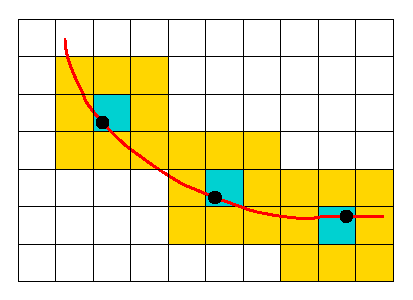
\includegraphics[width=0.4\linewidth]{images/selectA.eps} \qquad &
\qquad
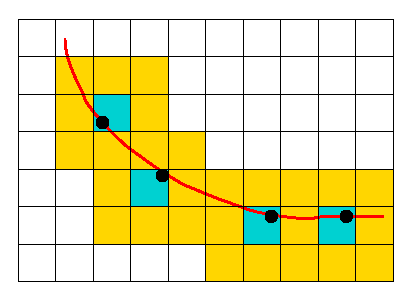
\includegraphics[width=0.4\linewidth]{images/selectB.eps} \\
(a) & (b)
\end{tabular}

\caption{2D illustration of vertex and cube selection.
(a) Selection which gives poor cover of the red curve.
The curve intersects an uncovered square.
(b) Selection which gives better cover of the red curve.
The curve is far away from any uncovered square.
}
\label{fig:select}
\end{figure}

\section{MergeSharp}

As show in Figure~\ref{alg:mergesharp}, Algorithm SHREC has three parts:
computation of isosurface vertex locations, 
selection of a well-spaced subset of vertices on sharp features
and merging of vertices around selected vertices.
Algorithm MergeSharp has a similar three parts,
but each part is substantially improved in SHREC.
We start with a brief description of MergeSharp
as presented in~\cite{bw-cisec-13}.

The computation of isosurface vertex locations
was described in Section~\ref{section:loc}.
The procedure in Section~\ref{section:loc}
returns not only a point $p_\cb$ on the isosurface,
but whether $p_\cb$ lies on a sharp corner, sharp edge or smooth portion 
of the isosurface.
Let $\Ccorner$ and $\Cedge$ be lists of cubes $\cb$ 
whose generated points $p_\cb$ lie on sharp corners and sharp edges, 
respectively.

As defined in Section~\ref{section:loc},
point $q_\cb$ is the centroid of interpolated intersection points
of the isosurface and grid edges of $\cb$.
Sort lists $\Ccorner$ and $\Cedge$ by increasing distance $|p_\cb - q_\cb|$
from $p_\cb$ to $q_\cb$.
Mark all the cubes as ``uncovered''.
Select the next uncovered cube $\cb$ in $\Ccorner$
where $p_\cb$ does not form a large angle triangle 
with vertices in previously selected cubes.
Merge $\cb$ with every uncovered vertex neighbor.
Mark all vertex neighbors of $\cb$ as covered.
The algorithm for $\Ccorner$ is shown in Figure~\ref{alg:select}.
After processing list $\Ccorner$, apply the same procedure to list $\Cedge$.

Note that the selection and merging are combined in the above description,
just as they are combined in~\cite{bw-cisec-13}.
In the modified version we present here,
those two steps will be separated.

There are problems with every one of the three steps of MergeSharp.
First, the vertex location $p_\cb$ generated by cube $\cb$
may lie outside $\cb$.
Moreover, point $p_\cb$ may lie outside of $\cb$
even if the sharp edge containing $p_\cb$ intersects $\cb$.
In addition, because of curvature, noise and numerical instability,
point $p_\cb$ could lie in some cube $\cb'$ adjacent to $\cb$
while point $p_{\cb'}$ lies inside $\cb$.
We will modify MergeSharp to generate point $p_\cb$ inside cube $\cb$
wherever possible.

Second, the selection step chooses cubes based on the proximity
of $p_\cb$ to $q_\cb$.
If a point $p_\cb$ is near $q_\cb$, 
it probably is located in cube $\cb$ 
and is a good approximation of the vertex location.
While this is reasonable,
it ignores the interaction between selected cubes.
MergeSharp does better when sharp edges are well-covered 
by the selected and covered cubes.
For instance, in the 2D illustration in Figure~\ref{fig:select}, 
the selected squares are packed together more closely
and their $3 \times 3$ regions do a better job of covering
the given curve.
We modified the MergeSharp selection to pack selected cubes 
more closely together.

Finally, the merging step merges cube $\cb$
with the the first selected cube adjacent to $\cb$.
Doing so sometimes distorts triangles, creating extremely thin triangles
and sometimes creating ``folds'' in the surface mesh.
We modify MergeSharp so that it prefers merging cubes which are facet
adjacent over merging edge adjacent or vertex adjacent cubes.
We add checks which avoid merging which creates small thin triangles
or creates folds.
We also extend the merging by one more cube in certain regions
to ensure good covering of sharp isosurface edges.


\begin{figure}[t]
\centering

\begin{tabular}{cc}
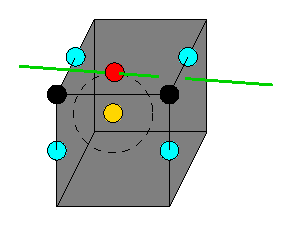
\includegraphics[width=0.4\linewidth]{images/centroid.eps} \qquad &
\qquad
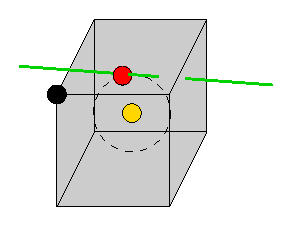
\includegraphics[width=0.4\linewidth]{images/center.eps} \\
(a) & (b)
\end{tabular}

\caption{The green line is the line containing the
sharp edge near cube $\cb$. 
Black cube vertices have scalar value above the isovalue.
(a) Green line intersects cube $\cb$
but point location $p^0_\cb$ (red) is outside cube $\cb$.
Cyan points are the intersection points of the isosurface
and the cube edges, computed using linear interpolation.
Gold point is $q_\cb$, the centroid of the cyan points, .
Red point is the closest point on the green line to $q_\cb$.
(b) Green line intersects cube $\cb$
but point location $p^1_\cb$ (red) is outside cube $\cb$.
Gold point is $\cb.\protect\Center$, the cube center.
Red point is the closest point on the green line to $\cb.\protect\Center$.
}
\label{fig:out_of_cube}
\end{figure}

\section{Generating Points on Sharp Features}
\label{section:generation}

\subsection{Computing Vertex Locations on Sharp Edges}

Consider an edge cube $\cb$.
By definition, edge cube $\cb$ is near some sharp edge.
The location $\cb.\isovLoc$ of the isosurface vertex associated with $\cb$ 
should be on that sharp edge.
However, that condition still gives one degree of freedom in selecting
the location of $\cb.\isovLoc$.
One obvious additional condition is that if the sharp edge intersects $\cb$,
then $\cb.\isovLoc$ should be in $\cb$.
An additional condition is that if the sharp edge does not intersect $\cb$,
then $\cb.\isovLoc$ should be ``close to'' $\cb$ 
under some suitably defined metric.

Algorithm SHREC computes three different possible isosurface vertex locations.
First, Algorithm SHREC computes $p^0_\cb$ 
by computing a line $L$ through the sharp edge and 
selecting the point on $L$ nearest the centroid point $q_\cb$.
Equation~\ref{eqn:Lindstrom}, for computing $p^0_\cb$ is given
in Section~\ref{section:loc}.
The idea is that the centroid point $q_\cb$ is a good approximation
for the intersection of $\cb$ and the isosurface,
and so one should choose a point near $q_\cb$.
If $p^0_\cb$ lies in $\cb$, then SHREC sets $\cb.\isovLoc$ to $p^0_\cb$.

In most cases, if line $L$ intersects cube $\cb$.
then the point $p^0_\cb$ will lie in $\cb$.
However, if line $L$ is ``near'' some facet or edge of $\cb$,
then it is possible for $L$ to intersect $\cb$ but $p^0_\cb$ to lie
outside $\cb$.
(See Figure~\ref{fig:out_of_cube}(a).)

If $p^0_\cb$ lies outside $\cb$,
then let $p^1_\cb$ be the point on $L$ which lies closest 
to the center $\cb.\Center$ of cube $\cb$.
We can compute $p^1_\cb$ replacing $q_\cb$ by $\cb.\Center$
in Equation~\ref{eqn:Lindstrom}.
If $p^1_\cb$ is in $\cb$ while $p^0_\cb$ is not,
SHREC sets $\cb.\isovLoc$ to $p^1_\cb$.

Unfortunately, it is possible that both $p^0_\cb$ and $p^1_\cb$ 
are not in $\cb$ even though $L$ intersects $\cb$.
(See Figure~\ref{fig:out_of_cube}(b).)
As a final step, we compute the point $p^2_\cb$ on $L$ which is closest 
to the center $\cb.\Center$ of $\cb$ under the $L_\infty$ metric.
If $L$ intersects $\cb$, then this point is guaranteed to lie in $\cb$.
Details for computing $p^2_\cb$ are in Appendix~\ref{appendix:Linf}.
If $p^2_\cb$ is in $\cb$ while $p^0_\cb$ and $p^1_\cb$ are not,
SHREC sets $\cb.\isovLoc$ to $p^2_\cb$.

Instead of computing $p^0_\cb$, $p^1_\cb$ and $p^2_\cb$, 
we could compute and use only $p^2_\cb$.
However, the computations of $p^0_\cb$ and $p^1_\cb$ are much faster,
and their locations are preferable to $p^2_\cb$ when they are
contained in cube $\cb$.
Algorithm MergeSharp computes only $p^0_\cb$.

\begin{figure}[t]
\centering

\begin{tabular}{cc}
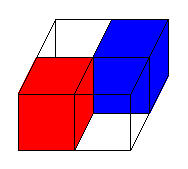
\includegraphics[width=0.4\linewidth]{images/shared_edge.eps} \qquad &
\qquad
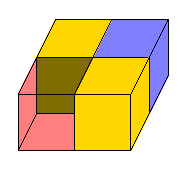
\includegraphics[width=0.4\linewidth]{images/shared_edge_B.eps} \\
(a) & (b)
\end{tabular}

\caption{(a) Two grids cubes sharing an edge $\eb$.
(b) The two other cubes (gold) which also contain $\eb$.
}
\label{fig:shared_edge}
\end{figure}

\begin{figure}[t]
\centering

\begin{tabular}{cc}
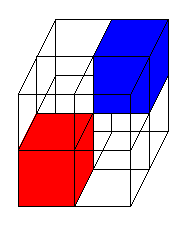
\includegraphics[width=0.4\linewidth]{images/shared_vertex.eps} \qquad &
\qquad
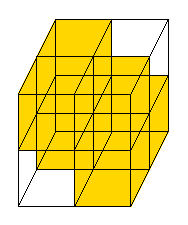
\includegraphics[width=0.4\linewidth]{images/shared_vertex_B.eps} \\
(a) & (b)
\end{tabular}

\caption{(a) Two grids cubes sharing a vertex $v$.
(b) The six other cubes (gold) which also contain $v$.
}
\label{fig:shared_vertex}
\end{figure}

\subsection{Swapping Locations}

Many of the problems in Algorithm SHREC (and MergeSharp) occur when
isosurface vertex location $\cb.\isovLoc$ lies outside of cube $\cb$.
Thus, it is always preferable that $\cb.\isovLoc$ be in $\cb$.
This is not always possible since the sharp edge or corner near $\cb$
may not intersect $\cb$.
However, in cases where a sharp edge or corner intersects $\cb$,
we would like $\cb.\isovLoc$ to be in $\cb$.

The computation of a sharp edge or corner near $\cb$ depends
upon gradients in the neighborhood of $\cb$.
The set of such gradients changes for each cube $\cb$.
Because of the inaccuracy in computing sharp edges and corners,
it is possible that $\cb.\isovLoc$ is in a cube $\cb'$ adjacent to $\cb$
while $\cb'.\isovLoc$ is not contained in $\cb$.
In some cases,
location $\cb.\isovLoc$ is in $\cb'$ while $\cb'.\isovLoc$ is in $\cb$.
In those cases,
we simply swap $\cb.\isovLoc$ and $\cb'.\isovLoc$.
In other cases, location $\cb'.\isovLoc$ lies in some third cube $\cb''$.
In that case, we simply set $\cb'.\isovLoc$ to $\cb.\isovLoc$.

The setting of isosurface vertex locations from adjacent cubes
increases the number of cubes $\cb$ containing 
their associated vertext locations $\cb.\isovLoc$.
Note that if the initial location $\cb.\isovLoc$ lies in $\cb$,
then we never change $\cb.\isovLoc$.


\begin{figure}
\centering
\begin{tabular}{cc}
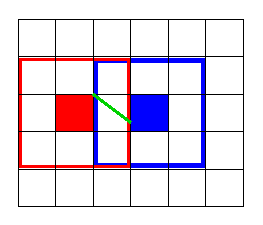
\includegraphics[width=1.2in]{images/config2D_2_0.eps} \qquad &
\qquad
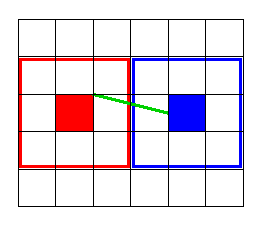
\includegraphics[width=1.2in]{images/config2D_3_0.eps} \\
(a) Configuration (2,0). & (b) Configuration (3,0). \\
\\
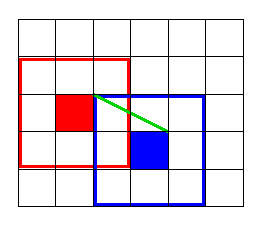
\includegraphics[width=1.2in]{images/config2D_2_1.eps}
\qquad &
\qquad
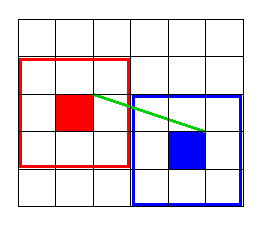
\includegraphics[width=1.2in]{images/config2D_3_1.eps} \\
(c) Configuration (2,1). & (d) Configuration (3,1).
\end{tabular}
\caption{Tightly packed 2D configurations of selected squares.
Selected squares and $3 \times 3$ region around each square.
Line segments with endpoints on the two selected squares 
(e.g., the green line segments) are contained
within the union of the two $3 \times 3$ regions.}
\label{fig:packed2D}
\end{figure}

\begin{figure}[t]
\centering
\begin{tabular}{cc}
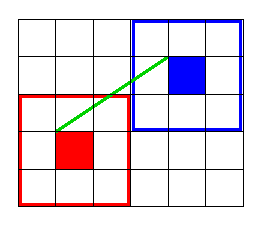
\includegraphics[width=1.2in]{images/config2D_3_2.eps} \qquad &
\qquad
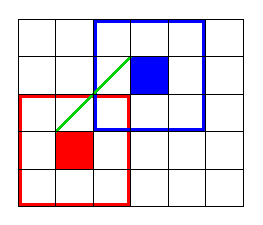
\includegraphics[width=1.2in]{images/config2D_2_2.eps} \\
(a) Configuration (3,2). & (b) Configuration (2,2). 
\end{tabular}
\caption{Problematic 2D configurations of selected squares.
Selected squares and $3 \times 3$ region around each square.
(a) The green line segment is not contained within the union
of the two $3 \times 3$ regions.
(b)~The green line segment intersects the boundary
of the union of the two $3 \times 3$ regions.}
\label{fig:loose2D}
\end{figure}

\begin{figure}[t]
\centering
\begin{tabular}{cc}
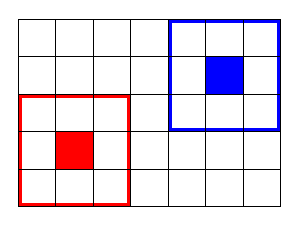
\includegraphics[width=1.2in]{images/config2D_4_2.eps} \qquad &
\qquad
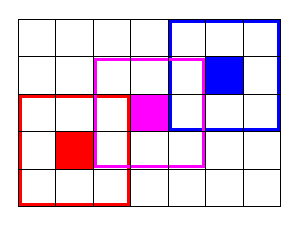
\includegraphics[width=1.2in]{images/config2D_4_2_B.eps} \\
(a) Configuration (4,2). & (b) Additional cube.
\end{tabular}
\caption{(a) Configuration (4,2) has space between the $3 \times 3$
regions around each selected square.
(b) Additional cube (magenta) which packs tightly with two other squares.}
\label{fig:config2D_4_2}
\end{figure}

\begin{figure*}
\centering
\begin{tabular}{cccc}
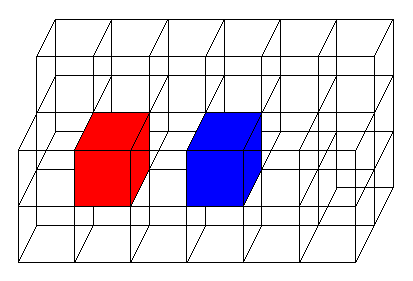
\includegraphics[width=1.2in]{images/config3D_2_0_0.eps} \qquad &
\qquad
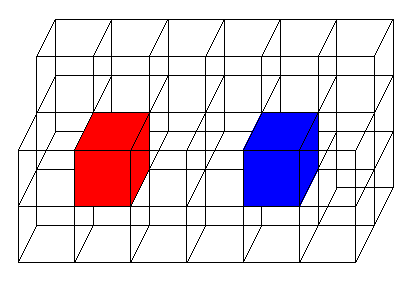
\includegraphics[width=1.2in]{images/config3D_3_0_0.eps}
\qquad &
\qquad
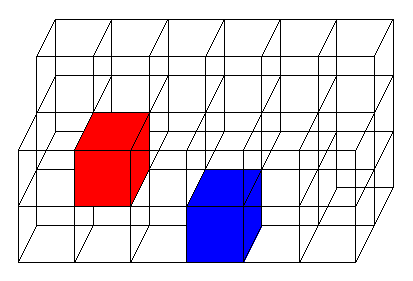
\includegraphics[width=1.2in]{images/config3D_2_1_0.eps}
\qquad &
\qquad
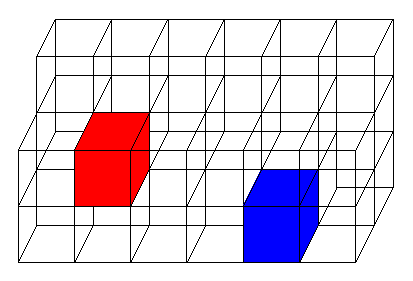
\includegraphics[width=1.2in]{images/config3D_3_1_0.eps} \\
(a) Configuration (2,0,0). & (b) Configuration (3,0,0). 
  & (c) Configuration (2,1,0). & (d) Configuration (3,1,0).
\end{tabular}
\caption{Tightly packed 3D configurations of selected cubes.}
\label{fig:packed3D}
\end{figure*}

\begin{figure*}
\centering
\begin{tabular}{ccc}
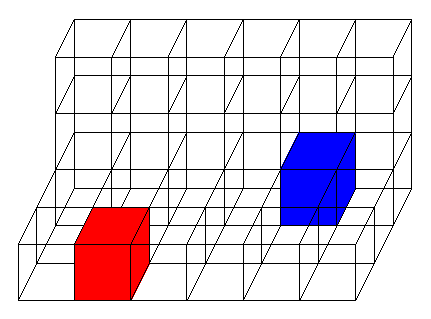
\includegraphics[width=1.2in]{images/config3D_3_2_0.eps} \qquad &
\qquad
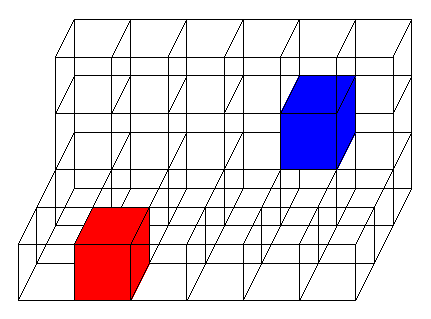
\includegraphics[width=1.2in]{images/config3D_3_2_1.eps}
\qquad &
\qquad
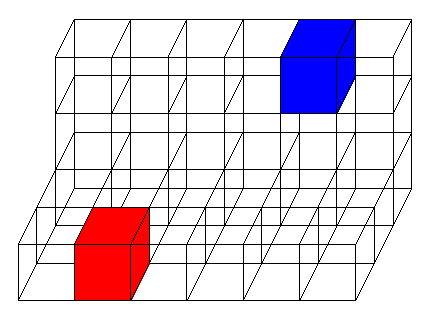
\includegraphics[width=1.2in]{images/config3D_3_2_2.eps} \\
(a) Configuration (3,2,0). & (b) Configuration (3,2,1). 
  & (c) Configuration (3,2,2).
\end{tabular}
\caption{Problematic 3D configurations of selected cubes.}
\label{fig:loose3D}
\end{figure*}

\begin{figure}[t]
\centering

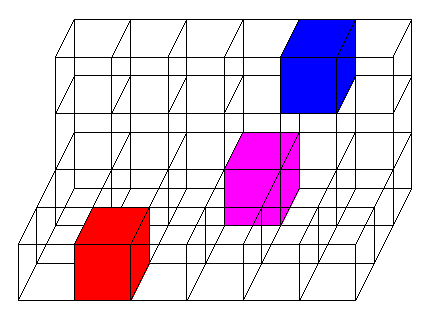
\includegraphics[width=1.2in]{images/config3D_3_2_2_B.eps}

\caption{Problematic interaction of red and blue cubes
in configuration (3,2,2) is blocked by magenta cube.}
\label{fig:blocked3D}
\end{figure}

\subsection{Locations on Planes}

Consider two grid cubes, $\cb$ and $\cb'$, 
which intersect in an edge $\eb$ but not in any facet.
(See Figure~\ref{fig:shared_edge}.)
Two other grid cubes, $\tcb$ and $\tcb'$ share edge $\eb$.
A sharp edge which passes through $\cb$ and $\cb'$ must intersect
either $\tcb$ or $\tcb'$.
(In the exceptional case, the edge passes through $\eb$,
in which case it intersects both $\tcb$ and $\tcb'$.)
Since the edge intersects either $\tcb$ and $\tcb'$,
either $\tcb.\isovLoc$ should be in $\tcb$ 
or $\tcb'.\isovLoc$ should be in $\tcb'$.
However, because of inaccuracies in computing sharp edges and corners,
neither condition may hold.

To ensure that either $\tcb.\isovLoc$ lies in $\tcb$
or $\tcb'.\isovLoc$ lies in $\tcb'$,
Algorithm SHREC computes the plane $h$ containing $\eb$
and perpendicular to the line from $\cb.\Center$ to $\cb'.\Center$.
SHREC then computes the intersection of the line $L$ containing $\eb$
and plane $h$.
This intersections point, $p_I$, lies in either $\tcb$ or $\tcb'$.
If $p_I$ lies in $\tcb$ and $\tcb.\isovLoc$ is not in $\tcb$,
SHREC sets $\tcb.\isovLoc$ to $p_I$.
If $p_I$ lies in $\tcb'$ and $\tcb'.\isovLoc$ is not in $\tcb'$,
SHREC sets $\tcb'.\isovLoc$ to $p_I$.

Next consider the case of two grid cubes, $\cb$ and $\cb'$, 
which intersect in a vertex $v$ but not in any edge.
(See Figure~\ref{fig:shared_vertex}.)
Six other grid cubes share vertex $v$ with $\cb$ and $\cb'$.
A sharp edge which passes through $\cb$ and $\cb'$ must intersect
one of these six other grid cubes.
(In the exceptional case, the edge passes through $v$,
in which case all six.)
Since the edge intersects one of the six grid cubes,
point $\tcb.\isovLoc$ should lie in $\tcb$ for one of the six grid cubes $\tcb$.
Again because of inaccuracies in computing sharp edges and corners,
point $\tcb.\isovLoc$ may not be in $\tcb$ for any of the six grid cubes $\tcb$.

To ensure that $p_\tcb$ lies in $\tcb$ for one of the six grid cubes,
Algorithm SHREC computes the plane $h$ containing $v$
and perpendicular to the line from $\cb.\Center$ to $\cb'.\Center$.
SHREC then computes the intersection of the line $L$ containing $\eb$
and plane $h$.
This intersections point, $p_I$, lies in at least one of the six grid cubes.
If $p_I$ lies in cube $\tcb$ and $\tcb.\isovLoc$ is not in $\tcb$,
SHREC sets $\tcb.\isovLoc$ to $p_I$.

The computation in this section ensures ``continuity'' in the cubes
which intersect a sharp edge.
If a sharp edge intersects a cube $\cb$,
then the edge should intersect two cubes $\cb'$ and $\cb''$
which share a facet with $\cb$.
SHREC's computation of edge-plane intersections described above,
ensures that if $\cb'$ and $\cb''$ are active cubes,
then $\cb'$ will contain $\cb'.\isovLoc$ and 
$\cb''$ will contain $\cb''.\isovLoc$.


\section{Selecting Edge and Corner Cubes}
\label{section:selection}

Algorithm SHREC selects a well-spaced subset of the edge and corner cubes
and merges isosurface vertices adjacent cubes 
with the vertices generated by the selected cubes.
To ensure that the isosurface vertices on sharp features are well-spaced,
SHREC never selects two cubes which have a common vertex.
Whenever SHREC selects a cube $\cb$,
any adjacent cube sharing a vertex with $\cb$ is marked as ``covered''
by $\cb$.
SHREC never selects a covered cube.

As noted in Section~???, 
SHREC does better when selected cubes 
are packed ``tightly'' together.
In particular, SHREC tries to avoid certain configurations of nearby cubes.

Consider cubes $\cb$ and $\cb'$ with grid indices $(x_0,x_1,x_2)$
and $(x'_0,x'_1,x'_2)$, respectively.
(A cube with grid indices $(x_0,x_1,x_2)$ is in column $x_0$, row $x_1$
and $z$-plane $x_2$ of the grid.)
The {\em distance vector} between the cubes is
$(|x_0-x'_0|, |x_1-x'_1|, |x_2-x'_2|)$.
Two grid cubes are in configuration $(a_0,a_1,a_2)$ if the distance vector
between the cubes is some permutation of $(a_0,a_1,a_2)$.
Figures~\ref{fig:packed2D}, \ref{fig:loose2D}, \ref{fig:config2D_4_2}
and~\ref{fig:packed3D},
contain examples of 2D and 3D configurations of grid cubes.

We can get some insight into 3D configurations of grid cubes
by considering the 2D configurations of grid squares.
Figure~\ref{fig:packed2D} contains configurations $(2,0)$, $(3,0)$,
$(2,1)$ and $(3,1)$ of grid squares.
The $3 \times 3$ regions around the selected squares are ``tightly packed''
so that any line segment with endpoints in the selected squares
is contained within the union of the two $3 \times 3$ regions.

Figure~\ref{fig:loose2D} contains configurations $(3,2)$ and $(2,2)$
of grid squares.
With configuration $(3,2)$, some line segments with endpoints
in the selected squares are not contained within the union
of the $3 \times 3$ regions.
Configuration $(2,2)$ is somewhat better,
since all line segments with endpoints in the selected squares
are contained within the union of the $3 \times 3$ regions.
Unfortunately, they are only barely contained.
The green line segment in Figure~\ref{fig:loose2D}(b) intersects
the boundary of the $3 \times 3$ region.
Slightly curving the segment could mean that it no longer was contained
in the union.

Note that if selected squares are suitably far apart,
then additional squares can be selected between them.
For instance, a magenta square can be selected between the two colored squares
in Figure~\ref{fig:config2D_4_2}(a) and the $3 \times 3$ regions
will fit together tightly.

Some examples of tightly packed 3D configurations of cubes are given
in Figure~\ref{fig:packed3D}.
Any line segment with endpoints in the two selected cubes $\cb$ and $\cb'$
will be well contained within the union 
of the two $3 \times 3 \times 3$ regions, 
$\RIII_\cb$ and $\RIII_{\cb'}$, around $\cb$ and $\cb'$.

Figure~\ref{fig:loose3D} contains three problematic configurations,
$(3,2,0)$, $(3,2,1)$ and $(3,2,2)$,
of  selected cubes.
Line segments with endpoints in the two selected cubes $\cb$ and $\cb'$
may contain points outside $\RIII_\cb \cup \RIII_{\cb'}$.
SHREC attempts to avoid selecting cubes with these configurations.

If two selected cubes, $\cb$ and $\cb'$, 
are in configuration $(2,2,0)$, $(2,2,1)$ or $(2,2,2)$,
then a line segment with endpoints in $\cb$ and $\cb'$
could intersect the boundary of $\RIII_\cb \cup \RIII_{\cb'}$.
Such configurations are undesirable.
Unfortunately, we found that avoiding such configurations is too restrictive.

Consider two cubes, $\cb$ and $\cb''$ 
in a $(3,2,0)$, $(3,2,1)$ or $(3,2,2)$ configuration.
If a third selected cube $\cb'$ lies between $\cb$ and $\cb''$,
then the sharp edge will pass from $\cb$ to $\cb'$ to $\cb''$.
The selection of $\cb'$ ``blocks'' the problematic interaction 
of $\cb$ and $\cb''$.
If cubes $\cb$ and $\cb'$ are selected,
then SHREC will permit the selection of $\cb''$,
even though $\cb$ and $\cb''$ have a configuration $(3,2,*)$.
Figure~\ref{fig:blocked3D} contains an example of two cubes 
in a $(3,2,2)$ configuration and a third cube between them.

More formally,
let $\cb$, $\cb'$ and $\cb''$ be grid cubes with grid indices
$(x_0,x_1,x_2)$, $(x'_0,x'_1,x'_2)$ and $(x''_0,x''_1,x''_2)$, respectively.
Cube $\cb'$ {\em separates} $\cb$ from $\cb''$
if $x'_i \in [x_i,x''_i]$ for $i = 0,1,2$
and $x_i < x'_i < x''_i$ or $x_i > x'_i > x''_i$ for some $i$.
SHREC avoids selecting cube $\cb''$ if some already selected cube $\cb$
forms a $(3,2,0)$ or $(3,2,1)$ or $(3,2,2)$ configuration with $\cb''$
and no already selected cube separates $\cb$ from $\cb''$.

SHREC first selects corner cubes.
When the corner location is inside an active cube,
SHREC selects the active cube containing the corner.
When the corner location is not in an active cube,
SHREC selects the active cube ``closest'' to the corner location
by choosing the cube whose center has minimum $L_\infty$ distance
to the corner.

SHREC next selects edge cubes which are ``near'' the corner cubes,
i.e., they are contained in an $7 \times 7 \times 7$ region
around each corner cube.
Selecting edge cubes near corners poses special challenges
since there are multiple sharp edges ending at a corner.
Selecting a cube which is near two such sharp edges
can obscure one of the edges.

Let $\cb$ be a corner cube and let $\cb'$ be an edge cube
which is in a $(2,0,0)$, $(2,1,0)$ or $(2,1,1)$ configuration with $\cb$.
Let $\cb''$ be any cube sharing an edge or facet with $\cb'$
which is contained in the $5 \times 5 \times 5$ region
but is not covered by $\cb$.
If $\cb''$ is active and an edge cube,
then SHREC attempts to avoid selecting cube $\cb'$.

Once edge cubes near corners are selected,
SHREC could iterate by selecting uncovered edge cubes 
near already selected cubes.
If no uncovered edge cubes were near selected cubes,
SHREC could select an arbitrary uncovered edge cube
and extend the set of selected cubes from that cube.
By not selecting a cube $\cb''$ 
if it forms a $(3,2,0)$, $(3,2,1)$ or $(3,2,2)$
with an already selected cube $\cb$ 
(and is not separated by a selected cube from $\cb$,)
SHREC would produce a tight packing of selected cubes.

The algorithm outlined in the previous paragraph would produce
a good set of selected cubes but it is highly sequential.
One of the best aspects of the Marching Cubes and dual contouring algorithms
is their local, distributed, paralellizable nature.
Sequentially extending the set of selected cubes would totally destroy
that aspect of the algorithms.
Instead of selecting cubes using the sequential algorithm given above,
SHREC divides the regular grid 
into overlapping $6 \times 6 \times 6$ regions,
selects cubes from the boundaries of those regions and then from their interior.
The algorithm is completely local and easily distributed and parallelizable.

Each grid cube has an index $(x_0, x_1, x_2)$.
SHREC processes the grid cubes by reducing the indices modulo six
to $(x_0 \bmod 6, x_1 \bmod 6, x_2 \bmod 6)$.
SHREC first selects edge cubes with indices congruent to $(0,0,0)$ modulo six.
SHREC next selects edge cubes with indices congruent modulo six
to $(\pm 1,0,0)$ or $(0, \pm 1, 0)$ $(0, 0, \pm 1)$.
SHREC then selects edge cubes with indices congruent modulo six
to $(\pm 2,0,0)$ or $(0, \pm 2, 0)$ $(0, 0, \pm 2)$.
Finally, SHREC selects edge cubes with indices congruent modulo six
to $(3,0,0)$ or $(0, 3, 0)$ $(0, 0, 3)$.
SHREC does not select an edge cube $\cb$ if some already selected cube $\cb'$
forms configuration $(3,2,0)$, $(3,2,1)$ or $(3,2,2)$ with $\cb$
and no already selected cube separates $\cb$ from $\cb''$.

SHREC next selects edge cubes which are some permutation
of $(k_a,k_b,0)$ modulo six,
starting first with permutations of $(\pm 1, \pm 1, 0)$
and ending with permutations of $(3, 3, 0)$.
Finally, SHREC selects edge cubes which are permutations
$(k_a, k_b, k_c)$ modulo six,
starting first with permutations of $(\pm 1, \pm 1, \pm 1)$
and ending with $(3, 3, 3)$.

It is possible that the selection of two edge cubes $\cb$ and $\cb''$
at distance five apart can force the selection of an edge cube $\cb'$
which has a $(3,2,1)$ or $(3,2,2)$ configuration 
with either $\cb$ or $\cb''$.
This happens if the distance vector between $\cb$ and $\cb''$
is $(5,3,2)$.
Thus, in addition to avoiding $(3,2,*)$ configurations,
SHREC also avoids selecting two cubes, $\cb$ and $\cb''$, 
which form a $(5,3,2)$ configuration.
Of course, if $\cb$ and $\cb''$ are separated by some other selected cube,
then they can both be selected.

While the above rules select a set of cubes which almost completely cover
the sharp edges of a surface,
it is possible that the configuration restrictions leave a few areas uncovered.
Therefore, SHREC repeats the selection process to select any remaining
uncovered edge cubes but drops the configuration restrictions.


\section{Merging Points with Features Points}
\label{section:merging}

Algorithm MergeSharp merges neighbors of a selected cube $\cb$ 
with $\cb$ when $\cb$ is selected.
This merging step sometimes created extremely thin triangles and 
sometimes flips triangle orientations.
SHREC is much more careful about its cube merging.
SHREC also extends the merging to some cubes in a $5 \times 5 \times 5$ region 
around each selected cube.
Note that SHREC actually merges the isosurface vertices generated by the cubes,
not the cubes themselves.

SHREC first merges neighbors of selected corner cubes.
SHREC merges these neighbors in three steps.
First, for each selected corner cube $\cb$,
SHREC merges with $\cb$ the active cubes which share a facet with $\cb$.
Next, for each selected corner cube $\cb$,
SHREC merges with $\cb$ the active cubes which share an edge with $\cb$.
Finally, for each selected corner cube $\cb$,
SHREC merges with $\cb$ the active cubes which share a vertex with $\cb$.
Of course, once an active cube is merged with some selected cube,
it is never merged with any other cube.

SHREC next merges neighbors of selected corner cubes.
The procedure is similar to the one for corner cubes.
SHREC first merges active cubes which share a facet with a selected edge cube,
then merges active cubes which share an edge with a selected edge cube,
and finally merges active cubes which share a vertex 
with a selected edge cube.

\subsection{Merging Tests}
\label{section:merging_tests}

For both the corner cube and edge cube merging,
SHREC applies five different tests to avoid creating very thin triangles
or flipping triangles or violating manifold conditions.
Consider a cube $\tcb$ which SHREC would like to merge 
with a selected cube $\cb$.
First, SHREC checks that the isosurface vertex in $\tcb$
is connected to the isosurface vertex in $\cb$.
A cube $\tcb$ is connected to a selected cube $\cb$
if $\tcb$ shares an active facet with $\cb$
or some cube $\tcb'$ shares an active facet with $\tcb$ and
is merged with $\cb$.
(A facet is active if some facet vertex has scalar value greater than
or equal to the isovalue and some facet vertex has scalar value less
than the isovalue.)
If $\tcb$ is not connected with $\cb$, then $\tcb$ is not merged with $\cb$.

Second, SHREC checks for some manifold violations that
could be caused by merging $\tcb$ with $\cb$.
For each such selected cube $\cb' \neq \cb$ which is connected to $\tcb$,
SHREC checks if $\cb'$ is connected to $\cb$.
Let $\cb'$ be a selected cube which is connected to $\cb$ and $\tcb$.
Each active edge $\eb$ of $\tcb$ is dual to an isosurface quadrilateral
with a vertex in $\tcb$.
Let $\tcb_1$, $\tcb_2$, and $\tcb_3$ be the three other cubes containing $\eb$.
If some $\tcb_i$ merges with $\cb$ and another $\tcb_j$ merges with $\cb'$,
then merging $\tcb$ with $\cb$ collapses this quadrilateral to a triangle
or an edge.
However, if no isosurface quadrilateral dual to an active edge of $\tcb$
has vertices in $\tcb$, $\cb$ and $\cb'$,
then merging $\tcb$ with $\cb$ creates a non-manifold edge 
from $\cb$ to $\cb'$ with four incident polygons.
If some selected $\cb'$ is connected to both $\cb$ and $\tcb$,
but no isosurface quadrilateral has vertices in $\tcb$, $\cb$ and $\cb'$,
then SHREC does not merge $\tcb$ with $\cb$.

Third, SHREC checks whether mapping $\tcb$ to $\cb$
will create thin triangles between selected cubes.
If SHREC is connected to selected edge cubes $\cb$, $\cb'$ and $\cb''$
and $\cb''$ lies between $\cb$ and $\cb'$
(or $\cb'$ lies between $\cb$ and $\cb''$),
then mapping $\tcb$ to $\cb$ will create a thin triangle
with vertices in $\cb$, $\cb'$ and $\cb''$.
Let $\cb$, $\cb'$ and $\cb''$ be grid cubes with grid indices
$(x_0,x_1,x_2)$, $(x'_0,x'_1,x'_2)$ and $(x''_0,x''_1,x''_2)$, respectively.
If $(x''_0,x''_1,x''_2)$ is contained in the box with corners
$(x_0,x_1,x_2)$ and $(x'_0,x'_1,x'_2)$ and does not lie on any 
of the eight corners of that box,
then we say that $\cb''$ lies between $\cb$ and $\cb'$.
If $\tcb$ is connected to selected edge cubes $\cb$, $\cb'$ and $\cb''$,
and $\cb''$ lies between $\cb$ and $\cb'$,
then SHREC does not merge $\tcb$ with $\cb$.

Fourth, SHREC checks whether mapping $\tcb$ creates thin triangles
or flips triangles.
This test is described in Section~\ref{section:distortion_tests}.

Finally, SHREC checks whether cube $\tcb$ has more than one isosurface vertex.
If cube $\tcb$ has more than one isosurface vertex,
then it has at least one ambiguous facet.
(A facet is ambiguous if two diagonally opposite vertices have
scalar value above the isovalue while the other two vertices
have scalar value below the isovalue.)
Let $\tcb'$ be a cube sharing an ambiguous facet with $\tcb$.
If cube $\tcb$ has only one isosurface vertex and 
$\tcb'$ is not merged with $\cb$, then $\tcb$ is not merged with $\cb$.

A cube $\tcb$ may fail to merge with a selected cube $\cb$
because of some neighboring cube $\tcb'$
while $\tcb'$ fails to merge with $\cb$ because of $\tcb$.
Often this ``deadlocking'' arises when $\tcb$ and $\tcb'$ share
a common ambiguous facet.

After attempting to merge individual cubes,
SHREC tries to merge pairs $(\tcb,\tcb')$ of covered cubes with selected cubes.
The elements of the pairs should share a common facet or edge
and should both be covered by the selected cube $\cb$.
SHREC temporarily merges $\tcb$ with $\cb$,
and then applies all the above tests to $\tcb'$.
SHREC then temporarily merges $\tcb'$ with $\cb$,
and applies all the above tests to $\tcb$.
If both $\tcb$ and $\tcb'$ pass the tests,
then SHREC merges both of them with $\cb$.

As the merging proceeds,
it is possible that a cube which was previously unable 
to merge with any selected cube
is now able to merge with some such cube.
Thus, SHREC repeats the above above merging procedures 
on any covered, unmerged cubes.

\subsection{Extended Merging}
\label{section:extended_merging}

The merging of cubes in $3 \times 3 \times 3$ region
around each selected cube will clear most but not all of the vertices 
around sharp edges and corners.
There are multiple reasons that some vertices near sharp edges may remain.
First, the location of some vertex outside of $\RIII_\cb$
may stop some cube covered by $\cb$ from merging with $\cb$.
Second, if two selected $\cb$ and $\cb'$ are 
in a $(2,2,0)$ or $(2,2,1)$ or $(2,2,2)$ configuration, 
then a sharp edge with endpoints in $\cb$ and $\cb'$ can intersect
the boundary of the $\RIII_\cb \cup \RIII_{\cb'}$.
Vertices in uncovered can be arbitrarily close to such a sharp edge.
Third, while the selection step avoids most $(3,2,*)$ configurations,
it does not avoid all of them.
If $\cb$ and $\cb'$ are in a $(3,2,*)$ configurations,
then a sharp edge with endpoints in $\cb$ and $\cb'$ may contain points
outside of $\RIII_\cb \cup \RIII_{\cb'}$.

To handle such problems, SHREC extends the merging to cubes
in a $5 \times 5 \times 5$ region around each selected cube.









\subsection{Distortion Tests}
\label{section:distortion_tests}

Let $q$ be a quadrilateral dual to some active edge of $\tcb$.
Let $\tw$ be the vertex of $q$ which is generated by $\tcb$.
Quadrilateral $q$ can either be triangulated by adding a diagonal
incident on $\tw$ or by adding a diagonal connecting the neighbors
of $\tw$ in $q$.
Triangulating $\tw$ by adding a diagonal incident on $\tw$
places more restrictions on possible locations of $\tw$.
Since SHREC does not know how $q$ will be triangulated,
it assumes this more restrictive triangulation.

The diagonal of $q$ incident on $\tw$ splits $q$ into two triangles.
SHREC checks whether mapping $\tcb$ to $\cb$ will severely distort
either of those triangles.
Let $\tcb$, $\tcb'$ and $\tcb''$ be the cubes 
containing the triangle vertices.
SHREC only checks triangles where $\tcb'$ and $\tcb''$ 
are not covered or selected.

Let $\tw$, $\tw'$ and $\tw''$ be the vertices generated
by $\tcb$, $\tcb'$ and $\tcb''$.
Let $w$ be the vertex generated by selected cube $\cb$.
SHREC applies three tests to determine if mapping $\tw$ to $w$
severely distorts triangle $(\tw,\tw',\tw'')$.
The first test simply checks that the angles in the new triangle
are not very small.
If $\angle(w,\tw',\tw'')$ or $\angle(w,\tw'',\tw')$ is less than $5^\circ$,
then SHREC does not map $\tcb$ to $\cb$.

The second test checks whether mapping $\tw$ to $w$
significantly changes the normal of triangle $(\tw,\tw',\tw'')$.
If the angle between the normal of $(w, \tw', \tw'')$ is less than $30^\circ$,
then the triangle passes this test.

The third test checks the orientation of $(w, \tw', \tw'')$.
Let $\eb$ be the grid edge shared by cubes $\tcb$, $\tcb'$ and $\tcb''$.
Let $\pi(w)$, $\pi(\tw')$ and $\pi(\tw'')$ be the orthogonal projection
of $w$, $\tw'$ and $\tw''$, respectively, 
onto a plane $h$ perpendicular to $\eb$.
If the orientation of $\pi(w)$, $\pi(\tw')$ and $\pi(\tw'')$
matches the orientation of $\tcb$, $\tcb'$ and $\tcb''$ around $\eb$,
then triangle $(w,\tw',\tw'')$ passes the orientation test.

We require that a triangle pass either the normal or the orientation test,
not necessarily both test.
The original triangle $(\tw,\tw',\tw'')$ could have a normal which
is very far from the true surface normal.
In that case, we actually want the normal of triangle $(w, \tw', \tw'')$
to be far from the normal of triangle $(\tw, \tw', \tw'')$.
On the other hand,
the projected vertices $\pi(w)$, $\pi(\tw')$ and $\pi(\tw'')$
could be nearly collinear.
In that case, $\pi(w)$, $\pi(\tw')$ and $\pi(\tw'')$ could have
opposite orientation from $\tcb$, $\tcb'$ and $\tcb''$,
even though the normal of $(w,\tw',\tw'')$ is quite close
to the original.




\section{Parameters}
\label{section:parameters}

